\chapter{Herramienta $\mathtt{SAT\_Solver}$}

En el presente capítulo se expondrá una herramienta para resolver el famoso problema de satisfacibilidad o más conocido como el problema $SAT$. Dicha herramienta se basará en la teoría presentada en los capítulos anteriores, mostrando así una de sus más relevantes aplicaciones. \\

Antes de tratar la herramienta, se pondrá al lector en situación dando una descripción detallada del problema de satisfacibilidad booleana; así como de su importancia, tanto para la comunidad científica internacional como para el resto de las personas.\\

Posteriormente, se describirán las tecnologías clave utilizadas en el desarrollo de la herramienta, que han dotado de estructura al proyecto además de concederle cierta robustez.\\

Finalmente, se realizará un análisis de eficiencia de la herramienta, durante el cual se detectaron ciertas ``fugas de tiempo''. Estas posibles mejoras se implementarán también dando lugar a una primera versión del \texttt{SAT-Solver}.

\newpage
\section{El problema $SAT$}

%\subsection{Definición}
Tal y como se definió en la página \pageref{def:sat}, una fórmula $F$ se dice \textit{satisfacible} si existe al menos una interpretación $i$ de $F$ que sea modelo de la fórmula. A partir de esta definición, es natural preguntarse cuándo una formula dada es satisfacible o no. Éste es el problema de la satisfacibilidad booleana o el comúnmente conocido como problema $SAT$. En definitiva consiste en saber \textit{a priori} si existe alguna forma de sustituir las variables proposicionales por $True$ o $False$, de manera que la fórmula sea verdadera. \\

Es importante destacar que para una fórmula con 10 variables, existen $2^{10} = 1024$ valoraciones a comprobar. Si a esto se suma que para que una fórmula se considere ``mínimamente interesante'' (en el mundo empresarial, por ejemplo) debe tener cientos de variables; el orden de magnitud de comprobaciones que se han de hacer es similar al número de átomos que hay en el universo. Este crecimiento tan rápido de combinaciones se debe a la complejidad exponencial intrínseca al problema de satisfacibilidad. \\

En teoría de la complejidad computacional, es considerado el problema capital de la clase de complejidad $NP$ al ser también un problema $NP$ duro ($NP$-hard), y ganándose así el estatus de problema $NP$-completo. \\

Respecto a los problemas $NP$-completos, no hay manera eficiente conocida de localizar una solución. Es decir, el tiempo requerido para resolver el problema usando cualquier algoritmo actualmente conocido aumenta muy rápidamente a medida que el tamaño del problema crece.\\

Como consecuencia, el problema de determinar si es posible resolver estos problemas de forma rápida, llamado problema $P$ versus $NP$ (¿$P=NP$?), es uno de los principales problemas sin resolver de la informática actual. Es por esto que en el año 2000, el \textit{Clay Mathematics Institute} lo declaró como el primer problema del milenio, junto a otros siete. Este título no es vano, ya que se cree que estos problemas marcarán el devenir de la comunidad científico-matemática.\\

Para comprender algo mejor la importancia del problema ¿$P=NP$? es importante conocer las consecuencias de su resolución. Si resultara que no son iguales, el impacto en la sociedad sería mínimo ya que únicamente se dejarían de buscar algoritmos de complejidad polinomial para resolver problemas de la clase $NP$.\\

Sin embargo, si se demostrase que ambas clases de complejidad son iguales, las implicaciones para la sociedad actual serían de una magnitud incomparable. Esto se debe a que la robustez de los sistemas criptográficos actuales se basan en la intratabilidad de ciertos problemas de la clase $NP$. Si éstos fueran resolubles en tiempo polinomial peligrarían todas las comunicaciones y las claves bancarias dejarían de ser seguras. Por otro lado, no todas las consecuencias son negativas ya que multitud de problemas de ámbito empresarial o social serían tratables; y por tanto, los costes se reducirían y los beneficios aumentarían.\\

Aunque, una vez vista la importancia del problema ¿$P=NP$? es natural preguntarse cómo podría resolverse. La respuesta es tan sencilla como dar un algoritmo que trabaje en tiempo polinomial en función del dato de entrada para un problema $NP$-completo, o demostrar que no existe dicho algoritmo. \\ 

El problema $NP$-completo objeto de la mayoría de estudios por parte de la comunidad científica es el problema $SAT$. Es tal su popularidad que cada año se publican multitud de nuevos algoritmos que dicen mejorar la eficiencia de resolución, y que se basan en las técnicas informáticas más innovadoras. \\

Con el objetivo de regular dicha competición, así como de identificar y promover nuevos retos relacionados con la resolución del problema $SAT$ surge la \textit{SAT Competition 2002}, enmarcada dentro del \textit{Fifth  International Symposium on the Theory and Applications of Satisfiability Testing}. Y desde ese año, de forma anual o bianual, se celebra tal competición. \\

Enmarcando el trabajo aquí presente en el contexto actual, éste pretende sentar las bases de un programa que resuelva el problema $SAT$ en un tiempo eficiente y que cumpla los estándares de dicha competición. Es por lo que a partir de este punto, la eficiencia será una máxima.\\

 Además, para poder participar en dicha competición se debe seguir un estándar, cuya regla principal es que la fórmula (o base de conocimiento) de entrada está escrita en un fichero de texto en forma normal conjuntiva utilizando el formato $DIMACS$ (se tratará con detalle más adelante).
 
 



%\subsection{Implicaciones}

\newpage

\section{Gestión del proyecto}
Es comúnmente aceptado que el proceso de creación de un programa consta de 5 etapas principales:

\begin{enumerate}
\item El desarrollo lógico del programa para resolver un problema en particular.
\item Escritura de la lógica del programa empleando un lenguaje de programación específico (codificación del programa).
\item Ensamblaje o compilación del programa hasta convertirlo en lenguaje de máquina.
\item Prueba y depuración del programa.
\item Desarrollo de la documentación.
\end{enumerate}

En esta sección se tratarán las tecnologías auxiliares usadas en las distintas etapas a fin de comprender su importancia dentro del proyecto, así como la necesidad (ya comentada anteriormente) de usar las herramientas que están a disposición del programador para desarrollar una aplicación de mayor calidad en menor tiempo.\\

El lenguaje de programación escogido es el lenguaje funcional Haskell, ya que encaja perfectamente con las necesidades del proyecto. Según la propia página web de Haskell, es un lenguaje que combina un fuerte sistema de tipos, inferencia de tipos y código de alto nivel, lo que afirman que ofrece al usuario la velocidad de desarrollo de lenguajes como Python o Ruby, además de una mayor robustez que lenguajes como Java o C++ .\\

A esto se le debe añadir que goza de una comunidad muy activa y un ecosistema de librerías muy rico, con multitud de librerías centradas en las matemáticas, y por ende, en los polinomios. Además, al ser objetivo del proyecto el definir diversas funciones matemáticas que actúen sobre el cuerpo $\mathbb{F} [\textbf{x}]$, resulta natural escoger un lenguaje funcional tipado.\\

En lo que refiere a la tercera etapa, destacar la herramienta \texttt{stack} que, definiendo una jerarquía específica de ficheros en nuestro proyecto, asiste el ensamblado y compilación. Esto permite usar el programa en cualquier computador sin la necesidad de instalar librerías auxiliares ya que con \texttt{stack} es suficiente. Sin embargo, el compilador primario que usa Haskell es GHC (Glasgow Haskell Compiler), un compilador en la vanguardia tecnológica, y de código libre, diseñado específicamente para Haskell.\\

Para la comprobación de la aplicación, el sistema de tipos de Haskell garantiza una cierta robustez, y es que asegura que cada función se utilice sobre los tipos para los que está diseñada. Por ejemplo, si intentamos calcular la suma de dos caracteres se devolverá un error al compilar.\\

Otro detalle a destacar de \texttt{stack} es que está diseñado de forma que la comprobación de los ejemplos sea muy natural y se haga automáticamente al compilar, con ayuda de la librería \texttt{doctest}. Cada vez que en el código hay ($>>>$) se ejecuta lo escrito a continuación y se corrobora si devuelve lo que aparezca en la línea siguiente (si es que se devolviese algo). Por ejemplo, en

\begin{code}
-- | 
-- >>> 2+2
-- 4
\end{code}

se comprueba si 2+2 devuelve 4. Notar que esto concede al proyecto de mucha robustez frente a modificaciones. Es decir, si se cambia el código de cierta función $f$ buscando una mayor eficiencia pero se comete algún error, se puede detectar al hacer las comprobaciones de los casos base, tanto de esta función como de alguna otra en la que intervenga $f$.\\

Otra ventaja, relacionada con las comprobaciones, que ofrece el lenguaje Haskell es la posibilidad de implementar propiedades matemáticas de las funciones o los tipos. Estas propiedades pueden ser esenciales en el desarrollo teórico pues pueden justificar, por ejemplo, la corrección de la aplicación o parte de ella.\\

Por lo tanto, es parte fundamental del proyecto verificar dichas propiedades mediante la librería \texttt{quickCheck}. Esta librería manda ejecutar 100 ejemplos y casos límites (el número 0, listas vacías, etc) para ver si sobre ellos se sigue verificando la propiedad. En el proyecto se comprobarán estas propiedades cada vez que se compile ya que junto a cada propiedad $prop$ se ha incluido:

\begin{code}
-- | 
-- >>> quickCheck prop
--  +++ OK, passed 100 tests
\end{code}

Así que, si en algún momento del desarrollo se deja de cumplir dicha propiedad para alguna instancia, el sistema devuelve el error.\\

En la etapa de documentación se ha utilizado una versión modificada del lenguaje Haskell, llamada Haskell literario. Ésta permite escribir código \LaTeX en el mismo archivo en el que se escribe el código Haskell. Por ejemplo, si se escribe en el archivo \texttt{.lhs}:

\begin{codigo}
Es un ejemplo
\begin{code}
ejemplo = "helloworld"
\end{code}
\end{codigo}

Al compilar se verá lo siguiente en el pdf:\\

Es un ejemplo
\begin{code}
ejemplo = "helloworld"
\end{code}

Con la ventaja principal de que la función $ejemplo$ se puede utilizar normalmente, como si se hubiese escrito en un archivo \texttt{.hs} típico.

Por último, se ha utilizado la herramienta \texttt{git} de control de versiones, que junto a la plataforma \texttt{GitHub} ha sido de gran ayuda en la depuración del código y la búsqueda de eficiencia.

\section{La herramienta}
A continuación, se describirán los distintos módulos de la herramienta, detallando los procesos más relevantes. Es importante destacar que los cálculos llevados a cabo por el programa se dividen principalmente en dos etapas:
\begin{enumerate}
\item Preprocesado del fichero de entrada.
\item Decisión por saturación con la regla de independencia.
\end{enumerate}

\subsection{Fichero de entrada y el formato \texttt{DIMACS}}
Previo a la descripción del formato \texttt{DIMACS} es necesaria una definición formal de qué es la forma normal conjuntiva. Con este objetivo se verán antes dos definiciones de la lógica proposicional.

\defn Un literal es una fórmula atómica o su negación. Se dice que un literal es \textit{positivo} si se trata de un átomo y \textit{negativo} si es la negación de un átomo.\\

Por ejemplo, $p_1$, $p_2$ ó $\neg p_1$ son literales.

\defn Una cláusula es una disyunción de literales. En otras palabras, es una colección finita de literales que se hace verdadera si alguno de ellos lo es. \\

Por ejemplo, $p_1 \vee p_2$ ó $p_1 \vee \neg p_2 \vee \neg p_3$ son cláusulas. Ya se está en condiciones de definir la forma normal conjuntiva.

\defn Dada una fórmula proposicional $F$ se dice que está en forma normal conjuntiva si se trata de una conjunción de cláusulas. \\

De cara al problema de satisfacibilidad es importante saber el que criterio debe cumplir una fórmula en forma normal conjuntiva para ser verdadera. Esta condición es que en todas sus cláusulas debe haber al menos un literal que sea verdadero.\\

Otra propiedad que se debe conocer sobre la forma normal conjuntiva es que dada cualquier fórmula proposicional existe otra equivalente en forma normal conjuntiva. El algoritmo \cite{apuntes} que la calcula es el siguiente:

\begin{center}
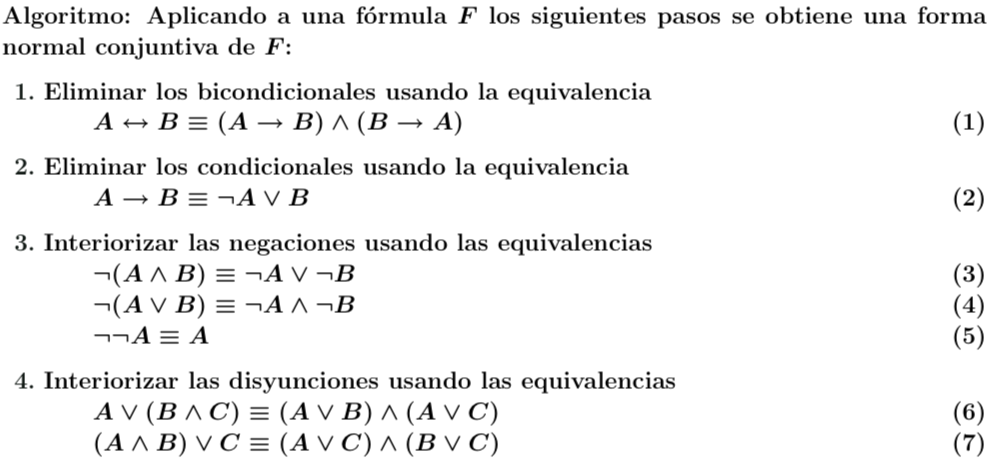
\includegraphics[scale=0.45]{imagenes/algfnc}
\end{center}

Como ya se ha comentado, se pretende presentar la herramienta a una competición, por tanto, debe cumplir ciertos requisitos para poder participar. El principal y más importante es que las instancias del problema $SAT$ que debe resolver vienen dadas en lo que se denomina el formato \texttt{DIMACS}. Un ejemplo de cómo se codificaría la fórmula $(p_1 \vee \neg p_5 \vee p_4)\wedge(\neg p_1 \vee p_5 \vee p_3 \vee p_4) \wedge (\neg p_3 \vee \neg p_4)$ en formato \texttt{DIMACS} es
\begin{table}[h]
\centering
\label{ej:dimacs}
\begin{tabular}{l}
{\Large \texttt{c} }\\\\
{\Large \texttt{c start with comments}} \\\\
{\Large \texttt{c}} \\\\
{\Large \texttt{c}}  \\\\
{\Large \texttt{p cnf 5 3}} \\\\
{\Large \texttt{1 -5 4 0}} \\\\
{\Large \texttt{-1 5 3 4 0}} \\\\
{\Large \texttt{-3 -4 0}}
\end{tabular}
\end{table}

Dicho formato es una estandarización simplificada de la forma normal conjuntiva de una fórmula. Las instancias serán archivos de texto (\texttt{.txt} o \texttt{.cnf}) con la siguiente estructura:

\begin{enumerate}
\item En primer lugar, se encuentran las líneas de comentarios. Se identifican gracias a que están encabezadas por la letra \texttt{c}. En el ejemplo, son las cuatro primeras líneas.
\item En segundo lugar, hay una línea distinguida que indica las propiedades de la fórmula como, por ejemplo, que está en forma normal conjuntiva (\texttt{cnf}). El segundo número que aparece indica cuántas variables proposicionales intervienen mientras que el segundo cuántas cláusulas.
\item Finalmente, en cada línea se encuentra codificada una cláusula distinta según las siguientes indicaciones:
\begin{itemize}
\item Cada número entero representa un literal.
\item El signo del número, positivo o negativo, indica si dicho literal es positivo o negativo, respectivamente.
\item El final de la cláusula se codifica con un 0.
\end{itemize} 
\end{enumerate}

\subsection{Preprocesado}

Las funciones que intervienen en el preprocesado tratan de transformar un archivo \texttt{.txt} ó \texttt{.cnf} en formato \texttt{DIMACS} al conjunto de polinomios que les corresponde según la función $\pi$. A continuación, se presentan estas funciones.

\entrada{Preprocesado}

\newpage
\subsection{Saturación}

Una vez que se tiene el conjunto de polinomios basta saturar dicho conjunto usando la regla de independencia. Las funciones encargadas de realizar este proceso son: \texttt{omiteVariableKB} y \texttt{saturaKB}. El módulo en el que se implementan estas se llama \texttt{Saturacion}.

\entrada{Saturacion}

Y así queda implementada una primera versión de la herramienta.

\newpage
\section{Análisis de la herramienta}

En esta sección se probará la herramienta con instancias de ejemplo, con el objetivo de detectar cotas de eficiencia. Las instancias se almacenan en el directorio \texttt{exDIMACS}, organizadas en carpetas según su dificultad.

\subsection{Directorio \texttt{easy}}
Este directorio contiene cuatro ejemplos muy sencillos, de hecho, las fórmulas que codifican sólo  tienen 2 variables ($p$ y $q$). El objetivo de estos ejemplos es servir como test para comprobar que el funcionamiento de la herramienta es el deseado.

\subsubsection{Ejemplo 1}

El archivo se llama \texttt{example1.txt}:
\begin{codigo}
c example 1 
c 
c f = (p ∨ q)
c
p cnf 2 1 
1 2 0
\end{codigo}

Y codifica la fórmula:
$$(p \vee q)$$

La ejecución en máquina es:
\begin{code}
>>> satSolver "exDIMACS/easy/example1.txt"
True
(0.00 secs, 586,368 bytes)
\end{code}
\subsubsection{Ejemplo 2}
El archivo se llama \texttt{example2.txt}:
\begin{codigo}
c example 2
c 
c f = (p ∨ q) ∧ (¬p ∨ q)
c
p cnf 2 2
1 2 0
-1 2 0
\end{codigo}

Y codifica la fórmula:
$$(p \vee q) \wedge (\neg p \vee q)$$

La ejecución en máquina es:
\begin{code}
>>> satSolver "exDIMACS/easy/example2.txt"
True
(0.00 secs, 792,784 bytes)
\end{code}
\subsubsection{Ejemplo 3}
El archivo se llama \texttt{example3.txt}:
\begin{codigo}
c example 3
c 
c f = (p ∨ q) ∧ (¬p ∨ q) ∧ (p ∨ ¬q)
c
p cnf 2 3
1 2 0
-1 2 0
1 -2 0
\end{codigo}

Y codifica la fórmula:
$$(p \vee q)\wedge (\neg p \vee q)\wedge ( p \vee \neg q)$$

La ejecución en máquina es:
\begin{code}
>>> satSolver "exDIMACS/easy/example3.txt"
True
(0.00 secs, 1,047,600 bytes)
\end{code}
\subsubsection{Ejemplo 4}
El archivo se llama \texttt{example4.txt}:
\begin{codigo}
c example 4
c 
c f = (p ∨ q) ∧ (¬p ∨ q) ∧ (p ∨ ¬q) ∧ (¬p ∨ ¬q)
c
p cnf 2 4
1 2 0
-1 2 0
1 -2 0
-1 -2 0
\end{codigo}

Y codifica la fórmula:
$$(p \vee q)\wedge (\neg p \vee q)\wedge ( p \vee \neg q)\wedge (\neg p \vee \neg q)$$

La ejecución en máquina es:
\begin{code}
>>> satSolver "exDIMACS/easy/example4.txt"
False
(0.01 secs, 1,361,672 bytes)
\end{code}

\newpage
\subsection{Directorio \texttt{medium}}
Tras comprobar que la herramienta responde de la forma deseada con los ejemplos anterior, conviene probar su eficiencia. Para ello, se construye una batería de ejemplos truncando el archivo \texttt{sat100.cnf} del directorio \texttt{hard}. Al ser conjuntos de cláusulas contenidas en un conjunto de cláusulas satisfacible son también satisfacibles y por tanto, el resultado de usar la herramienta debe ser \texttt{True}.

Únicamente se tratarán los tres primeros ejemplos ya que el resto no se ejecuta en un tiempo razonable.

\subsubsection{Ejemplo 0}
El archivo se llama \texttt{exampleSat0} y codifica una fórmula en forma normal conjuntiva con 30 cláusulas en las que intervienen hasta 59 variables distintas. Destacar que tanto en este ejemplo como en los próximos, en cada cláusula habrá exactamente 3 literales.

\begin{codigo}
c 
c    clause length = 3 
c
p cnf 59 30
30 -19 -3 0
89 31 -42 0
1 10 38 0
2 -21 -98 0
36 56 -78 0
14 -59 -87 0
89 -75 -86 0
-20 -80 4 0
-63 90 -55 0
59 75 9 0
-5 31 -97 0
48 -35 58 0
28 84 16 0
65 -4 94 0
-72 -23 7 0
18 -64 -55 0
-96 3 -35 0
89 -65 83 0
8 -60 -28 0
34 50 -14 0
64 -47 -35 0
-19 57 93 0
52 99 -94 0
-59 10 48 0
-78 -44 76 0
-63 -48 52 0
-88 84 -68 0
10 88 -76 0
92 -81 -88 0
\end{codigo}

La ejecución en máquina es:
\begin{code}
>>> satSolver "exDIMACS/medium/exampleSat0.txt"
True
(0.02 secs, 10,307,480 bytes)
\end{code}

\subsubsection{Ejemplo 5}
El archivo se llama \texttt{exampleSat1.txt} y codifica una fórmula satisfacible con 91 cláusulas y 82 variables. Por razones de espacio se omitirá mostar el archivo. La ejecución en máquina es:
\begin{code}
>>> satSolver "exDIMACS/medium/exampleSat1.txt"
True
(5.87 secs, 2,122,138,840 bytes)
\end{code}

\subsubsection{Ejemplo 6}
El archivo se llama \texttt{exampleSat2.txt} y codifica una fórmula satisfacible de mayor tamaño que la anterior, de hecho, la contiene. Por razones de espacio se omitirá mostar el archivo. La ejecución en máquina es:
\begin{code}
>>> satSolver "exDIMACS/medium/exampleSat2.txt"
True
(139.13 secs, 34,754,329,424 bytes)
\end{code}

\subsection{Directorio \texttt{hard}}

En este directorio se encuentras tres archivos \texttt{.cnf} que son tres ejemplos oficiales de instancias dadas por la organización de la competición $SAT$ en la que se pretende participar.

\subsubsection{Archivo \texttt{sat100.cnf}}
Este ejemplo consta de 100 variables en 430 cláusulas. La fórmula es satisfacible pero tiempo de ejecución sobrepasa la hora.
\subsubsection{Archivo \texttt{sat250.cnf}}
Este ejemplo consta de 250 variables en 1065 cláusulas. La fórmula es satisfacible aunque el tiempo de ejecución excede la hora.
\subsubsection{Archivo \texttt{unsat250.cnf}}
Este ejemplo consta de 250 variables en 1065 cláusulas. La fórmula es insatisfacible y la ejecución queda:
\begin{code}
>>> satSolver "exDIMACS/hard/unsat250.cnf"
False
(0.05 secs, 34,873,832 bytes)
\end{code}

\subsection{Heurísticas}
Ya en el ejemplo 5, el tiempo de ejecución es demasiado alto. Sin embargo, en el ejemplo 6 y posteriores (exceptuando \texttt{unsat250.cnf}) el coste en tiempo excede lo razonable, por lo que se pone de manifiesto la necesidad de una mejora en la implementación.\\

Tras diversas pruebas, la mejora que se ha implementado se debe al hecho observado de que aunque el resultado tras saturar permanezca invariante si se cambia el orden de las variables a omitir, el tiempo de ejecución sí cambia.\\

A raíz de esto se probarán experimentalmente varias heurísticas; y en base a estos experimentos, se escogerá la que tenga mejores resultados. Es importante tener en cuenta que no es seguro que el orden escogido sea el óptimo ya que nos basamos en un criterio absolutamente empírico.\\

Se define el módulo \texttt{Heuristicas}, en el que se implementarán dichas heurísticas.

\entrada{Heuristicas}

Quedando la resolución del ejemplo 5:

\begin{code}
>>> satSolver heuristicaLex "exDIMACS/medium/exampleSat1.txt"
True
(5.82 secs, 2,122,150,944 bytes)
>>> satSolver heuristicaFrecuencia "exDIMACS/medium/exampleSat1.txt"
True
(0.24 secs, 62,955,680 bytes)
>>> satSolver heuristicaFrecRev "exDIMACS/medium/exampleSat1.txt"
True
(7.08 secs, 3,372,336,472 bytes)
\end{code}

Mientras que la del ejemplo 6:

\begin{code}
>>> satSolver heuristicaLex "exDIMACS/medium/exampleSat2.txt"
True
(137.98 secs, 34,754,335,488 bytes)
>>> satSolver heuristicaFrecuencia "exDIMACS/medium/exampleSat2.txt"
True
(0.30 secs, 92,607,744 bytes)
>>> satSolver heuristicaFrecRev "exDIMACS/medium/exampleSat2.txt"
Interrupted.
\end{code}

Tras varios minutos de espera queda patente que la tercera heurística no es eficiente. Si se prueba la segunda (\texttt{heuristicaFrecuencia}) con el ejemplo 7 y con \texttt{unsat250.cnf}

\begin{code}
>>> satSolver heuristicaFrecuencia "exDIMACS/medium/exampleSat3.txt"
True
(5.87 secs, 2,317,863,248 bytes)
>>> satSolver heuristicaFrecuencia "exDIMACS/hard/unsat250.cnf"
False
(0.06 secs, 34,872,144 bytes)
\end{code}

En función de estos resultados, la heurística escogida es \texttt{heuristicaFrecuencia}. Sin embargo, el tiempo sigue siendo demasiado alto si se quiere resolver el ejemplo 8 o algunas de las dos instancias satisfacibles del directorio \texttt{hard}.